\documentclass[12pt,a4paper,portrait]{beamer}
\usetheme{default}
\usecolortheme{crane}
\usepackage{polski}
\usepackage[utf8]{inputenc}
\usepackage[polish]{babel}
\usepackage{amsmath}
\usepackage{amsfonts}
\usepackage{amssymb}
\usepackage{graphicx}
\usepackage{ragged2e}
\usepackage{multimedia}
%\usepackage{movie15}
%\usepackage{hyperref}
\usepackage{listings}

\author[AW]{Adam Wolniakowski}
\institute[WM PB]{Politechnika Białostocka}
\title[ROS]{Robot Operating System}
\date{30 października, 2014}
%\logo{\includegraphics[width=1cm]{logo.png}}

\begin{document}
\section{Start}
\begin{frame}
\titlepage
\end{frame}



\section{Wprowadzenie}
\begin{frame}
\frametitle{Co to jest ROS?}
ROS (\textit{Robot Operating System}) to open-source'owy, meta-system operacyjny, przeznaczony do zastosowań w robotyce.
Zapewnia to, czego można oczekiwać od systemu operacyjnego:
\begin{itemize}
\item abstrakcję hardware
\item kontrolę urządzeń na niskim poziomie
\item przekazywanie danych między procesami
\item komunikacja między różnymi hostami
\item $\cdots$
\end{itemize}
\end{frame}


\begin{frame}
\frametitle{\textit{Reinventing the wheel}}
\begin{center}
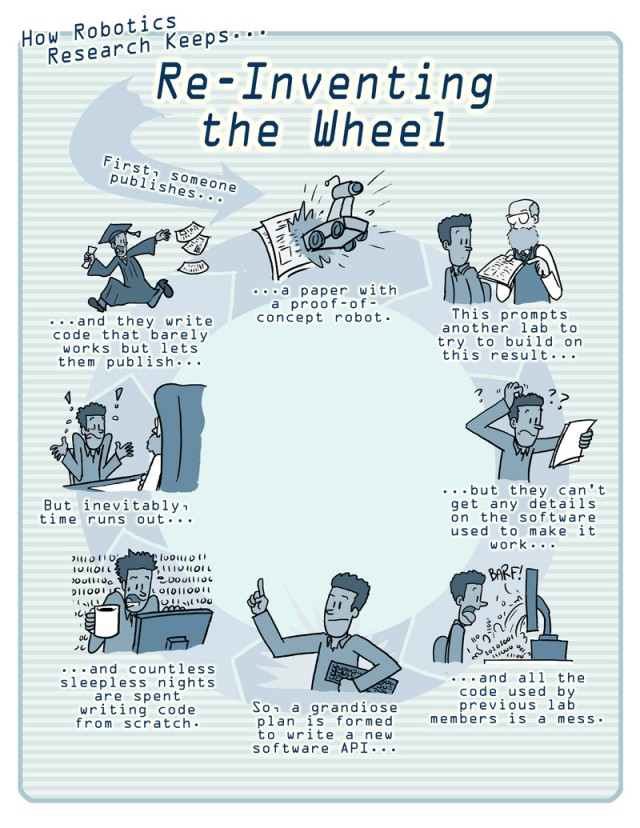
\includegraphics[width=0.6\textwidth]{pics/comic1.jpg}
\end{center}
\end{frame}


\begin{frame}
\frametitle{\textit{Willow Garage}}
\begin{center}
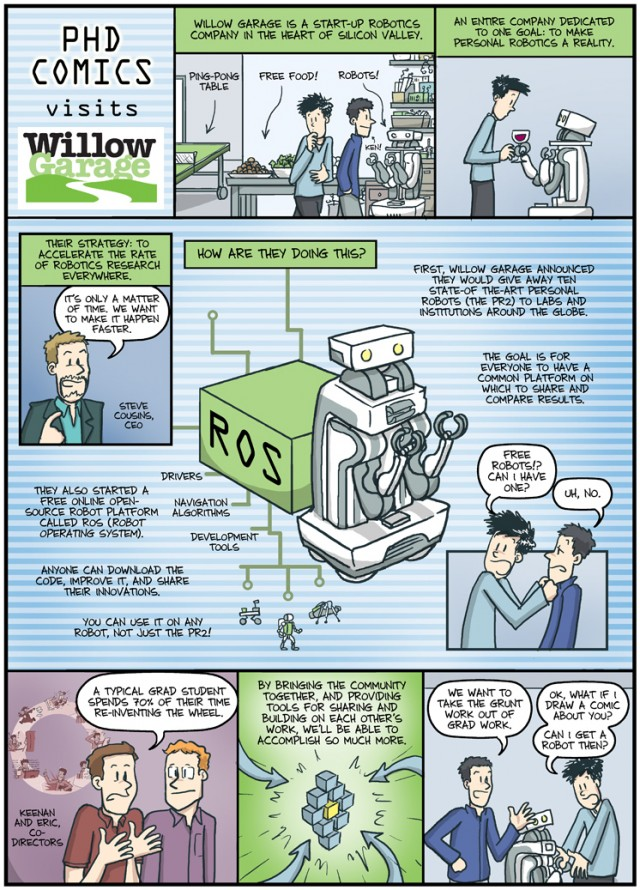
\includegraphics[width=0.5\textwidth]{pics/comic2.jpg}
\end{center}
\end{frame}


\begin{frame}
\frametitle{\textit{Why?}}
Dlaczego warto zastanowić się nad użyciem ROS-a?
\begin{itemize}
\item Nie ma sensu implementować wszystkiego od zera
\item Gotowe sterowniki dla wielu urządzeń
\item Bardzo aktywna społeczność
\item ROS jest fajny
\end{itemize}
\end{frame}


\begin{frame}
\frametitle{Paczki}
ROS integruje kilka interesujących rzeczy:
\begin{itemize}
\item OpenCV
\item PCL
\item SLAM
\item Sterowniki: Kinect, IMU, kamery, GPS, ...
\item Planowanie trajektorii
\item Symulatory
\end{itemize}
\end{frame}



\section{ROS}
\begin{frame}
\frametitle{POJĘCIA}
Poniżej spróbujemy wyjaśnić kilka podstawowych pojęć:
\begin{itemize}
\item node
\item message
\item topic
\item service
\end{itemize}
\end{frame}


\begin{frame}
\frametitle{Struktura ROS-a}
\textbf{ROS} jest zorientowany na komponenty.
\vspace{1cm}

Komponent ROS-a nazywamy \textit{node}. Komponenty komunikują się między sobą przy pomocy strumieni danych (\textit{topics}), lub wywołując usługi (\textit{services}).
\end{frame}


\begin{frame}
\frametitle{Node}
\textbf{Node} to komponent systemu. Każdy z nich może być uruchomiony oddzielnie, w dowolnym momencie, na dowolnym hoście. \textit{Node}-y posiadają wejścia i wyjścia.

Komponentem może być na przykład:
\begin{itemize}
\item sterownik robota
\item kamera
\item program odpowiedzialny za przetwarzanie danych
\item archiwum
\item ...
\end{itemize}
\end{frame}


\begin{frame}[fragile]
\frametitle{Message}
\textbf{Message} to pojedyncza ramka informacji przesyłana pomiędzy komponentami. ROS wyposażony jest w bogatą bibliotekę gotowych wiadomości (np. PCL, transformacje, macierze, obrazy, typy standardowe, ...). Wiadomości można też łatwo zdefiniować samemu.


\begin{block}{Format wiadomości}
\begin{verbatim}
#komentarz
float64 myDouble
string myString
float64[] myArrayOfDouble
\end{verbatim}
\end{block}
\end{frame}


\begin{frame}
\frametitle{Topic}
\textbf{Topic} jest strumieniem danych przekazywanych pomiędzy komponentami. Do jednego \textit{topic}-u mogą jednocześnie publikować i subskrybować dane różne komponenty.

\textit{Topic} to zazwyczaj dane publikowane regularnie.

\begin{center}
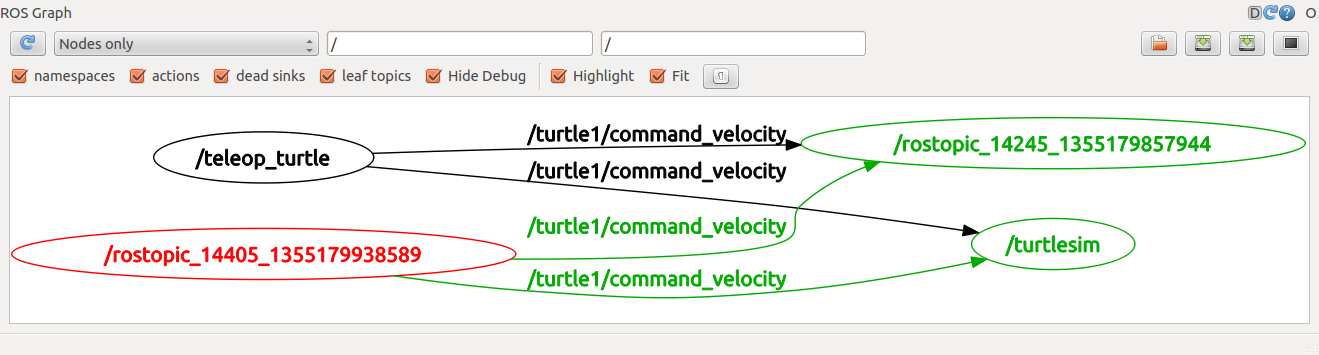
\includegraphics[width=1\textwidth]{pics/topic.png}
\end{center}
\end{frame}


\begin{frame}[fragile]
\frametitle{Service}
\textbf{Service} umożliwia wywołanie pewnej usługi, bądź komunikację asynchroniczną. Usługi można również definiować samodzielnie (format jest podobny do wiadomości).

\begin{block}{MyService.srv}
\begin{verbatim}
#wejscie
float64 dzielna
float64 dzielnik
---
#wyjscie
float64 iloraz
\end{verbatim}
\end{block}
\end{frame}



\section{Programowanie}
\begin{frame}
\frametitle{Języki programowania}
ROS sprawnie obsługuje następujące języki programowania:
\begin{itemize}
\item C / C++
\item Python
\item Java
\end{itemize}

Dodatkowo, można wykorzystać języki skryptowe (np. LUA), opisowe (XML), itd.
\end{frame}

\begin{frame}
\frametitle{Współpraca z Matlabem i Simulinkiem}
Można znaleźć toolboxy, które umożliwiają wykorzystanie systemu ROS z poziomu Matlaba, np. ROS IO toolbox.

\vspace{1cm}
Implementując odpowiednie funkcje MEX, można stworzyć bloki w Simulinku umożliwiające komunikację z systemem. Można w ten sposób zrealizować zapis danych i sterowanie w czasie rzeczywistym, budując odpowiedni model w Simulinku.
\end{frame}



\section{Bender}
\begin{frame}
\frametitle{Stanowisko 'Bender'}
Stanowisko badawcze w sali 608 `\textit{Na antresoli}' zawiera m.in. roboty UR5, kamery, TrakStar, chwytaki, ...


Docelowo ma być kopią stanowiska \textit{MARVIN} z uniwersytetu SDU w Odense.

\begin{center}
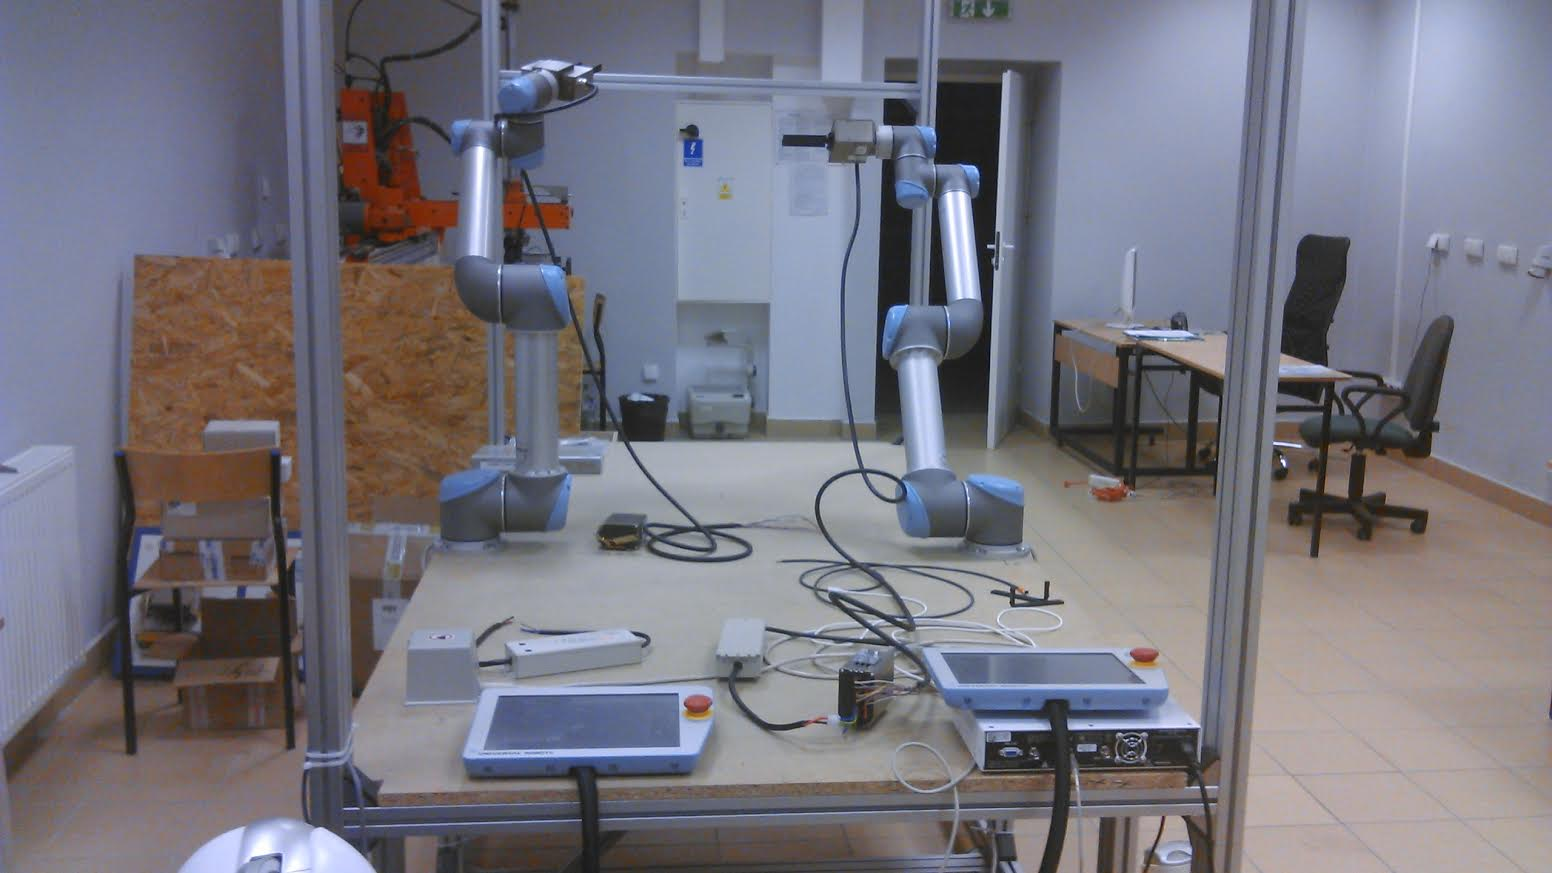
\includegraphics[width=0.67\textwidth]{pics/bender}
\end{center}
\end{frame}

\begin{frame}
\frametitle{Struktura}
Stanowisko \textit{Bender} będzie obsługiwane przez system ROS. Dla każdego z urządzeń zostanie zaimplementowany komponent ROS, co umożliwi łatwą obsługę stanowiska zarówno na miejscu, jak i zdalnie.

\begin{center}
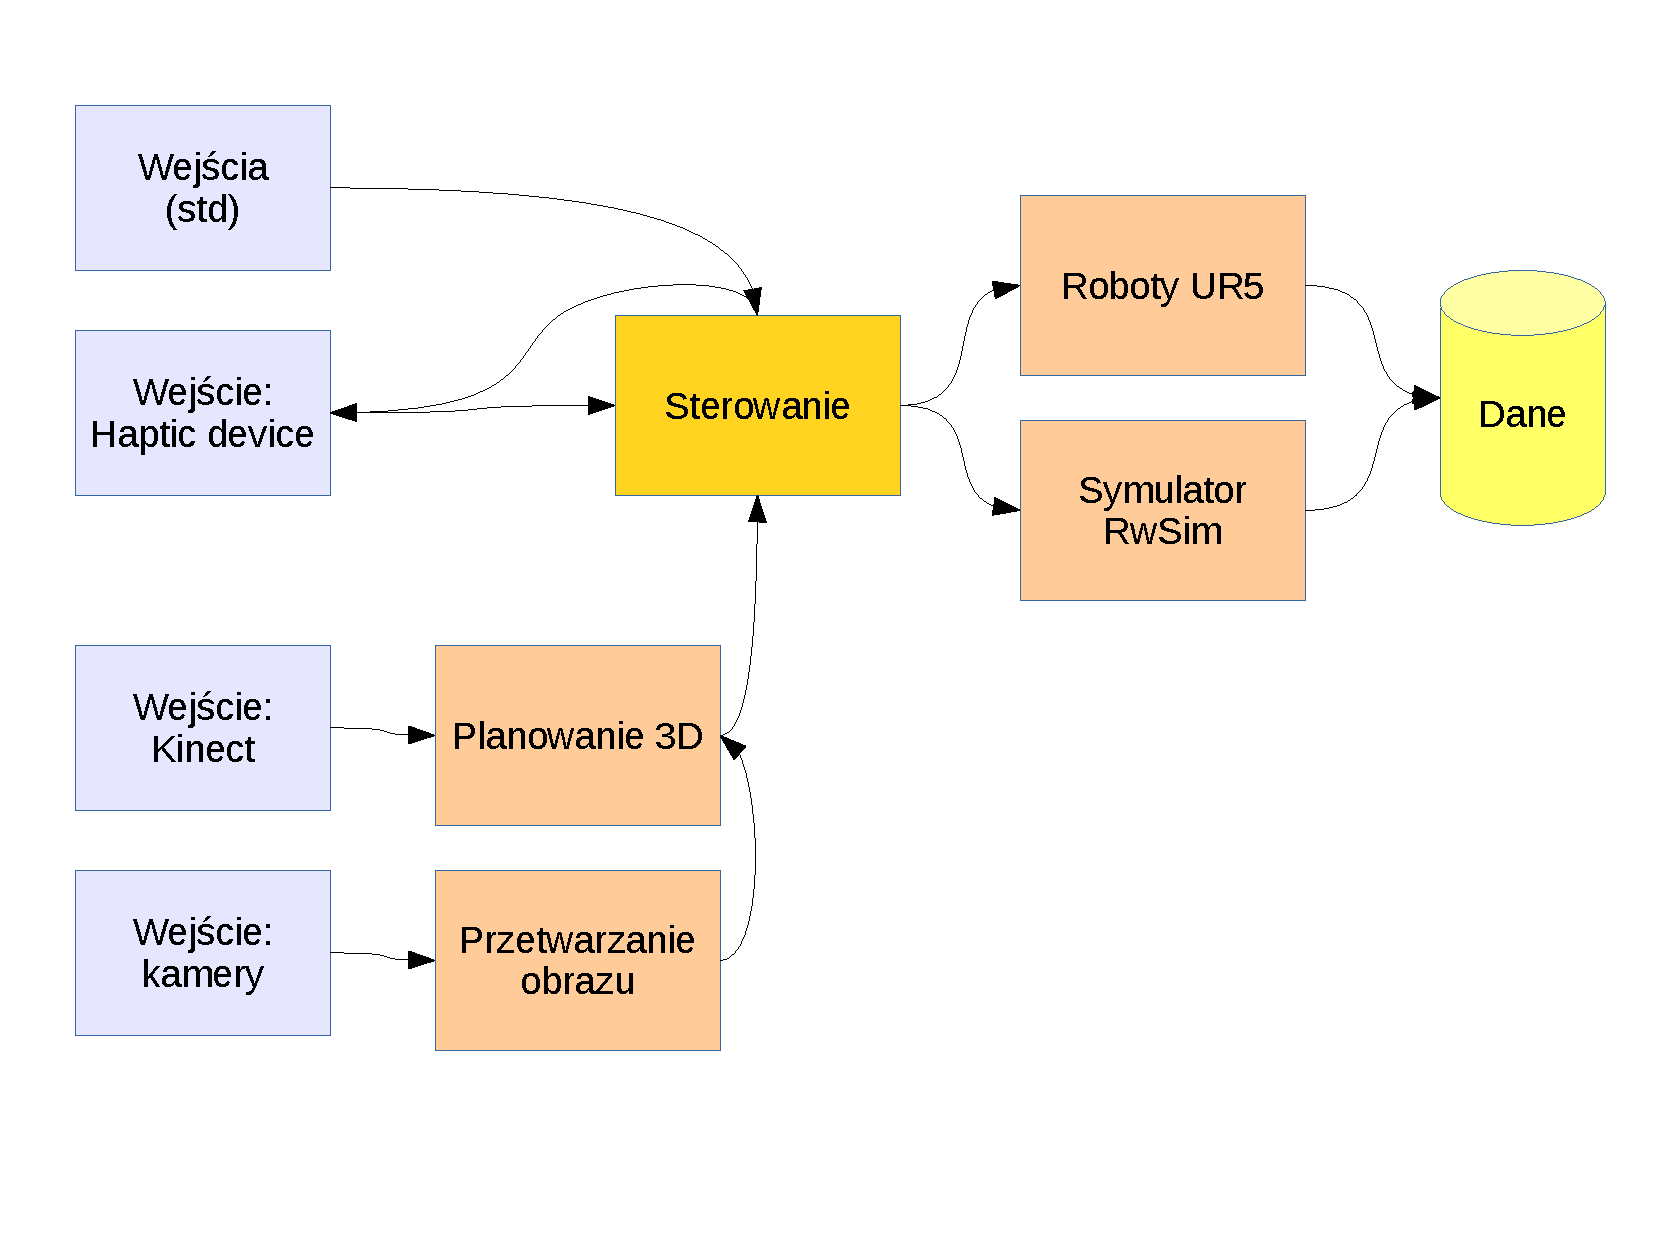
\includegraphics[width=0.67\textwidth]{pics/struktura.pdf}
\end{center}
\end{frame}



\section{Koniec}
\begin{frame}
\frametitle{Koniec}
Dziękuję! Nareszcie!
\end{frame}

\end{document}